% ============================================================================
% IBERAMIA resubmission — Springer LNCS format.
% Requires the Springer llncs.cls (not redistributable here). See README.md in
% this folder for how to obtain it, or switch \documentclass to `article` for a
% quick local preview (the content compiles either way with minor spacing diff).
% ============================================================================
\documentclass[runningheads]{llncs}

\usepackage[T1]{fontenc}
\usepackage[utf8]{inputenc}
\usepackage{graphicx}
\usepackage{amsmath,amssymb}
\usepackage{booktabs}
\usepackage{tabularx}
\usepackage{url}
\usepackage{xcolor}

% Placeholder macro for numbers to be filled after re-running the leakage-free
% pipeline (results/classification/summary.json -> paper/generated/*.tex).
\newcommand{\TODO}[1]{\textcolor{red}{\textbf{[#1]}}}

\begin{document}

\title{Do Synthetic Mammograms Really Help?\\
A Powered, Leakage-Free Evaluation of GAN and\\
Diffusion Augmentation for Breast Cancer Classification}
\titlerunning{Do Synthetic Mammograms Really Help? A Powered, Leakage-Free Evaluation}

\author{Rafael Palheta Tokairin\inst{1}\orcidID{0000-0000-0000-0000} \and
Helen C. de Mattos Senefonte\inst{1} \and
Neyva Maria Lopes Romeiro\inst{1}}
\authorrunning{R. P. Tokairin et al.}
\institute{State University of Londrina (UEL), Londrina, Brazil\\
\email{rafael.tokairin@uel.br}}

\maketitle

\begin{abstract}
Deep learning for mammography is limited by the scarcity of labelled data, and
generative models---GANs and, more recently, diffusion models---are a common
remedy. However, when the generator or the sample-selection step sees images
later used for evaluation, reported gains become optimistic, and studies are
often too small to be statistically powered. We present a \textbf{powered,
leakage-free, patient-level protocol} for measuring the effect of synthetic
mammograms on a downstream classifier, and apply it to \emph{two} generators: a
conditional StyleGAN2-ADA and a Stable-Diffusion-1.5 model fine-tuned with LoRA.
Using the \textbf{full CBIS-DDSM} (2857 full-mammogram images, 1460 patients),
we split at the patient level into a development pool and a \textbf{locked test
set of 504 images} (252/class, 290 patients) never seen by any generator or
selection filter, and evaluate EfficientNet-B0 over 10 seeds. Synthetic images
are perceptually filtered by an LPIPS sweep and audited for memorisation;
generative quality is reported with FID and KID. Effects relative to a real-only
baseline are assessed with Holm-corrected paired Wilcoxon tests, bootstrap
confidence intervals, Cliff's delta, and DeLong. Our central finding is a
\textbf{generator-agnostic null}: neither the GAN nor the diffusion model
improves classification over the real-only baseline (test AUC $0.733$); every
augmented ratio is statistically indistinguishable from it. Strikingly, the
diffusion generator is \emph{more} realistic (FID $131.3$/$126.1$ vs the GAN's
$158.7$/$171.6$), \emph{more} diverse, and shows \emph{zero} memorisation, yet
still yields no downstream benefit---so generator quality is \textbf{not} the
bottleneck. \textbf{External validation} on a second dataset (MIAS, no
retraining) confirms the model does not generalise (AUC near chance). Finally, a
nuanced leakage ablation shows the apparent positive result requires \emph{both}
a small subset \emph{and} image-level leakage: on the full, powered dataset even
the leaky image-level split is null. GAN augmentation also does not beat cheap
classic augmentation. We follow CLAIM and TRIPOD+AI reporting guidance; code and
the trained checkpoints are released.

\keywords{Synthetic data \and Generative adversarial networks \and Diffusion
models \and Mammography \and Data leakage \and Reproducibility \and Data
augmentation.}
\end{abstract}

% ============================================================================
\section{Introduction}
% ============================================================================
Breast cancer is the most common cancer among women, and mammography is the
primary screening modality~\cite{precoce2004controle,azevedo2016importancia}.
Manual interpretation is subject to inter-observer variability and
fatigue~\cite{obuchowicz2020interobserver}, motivating computer-aided
tools. Convolutional neural networks (CNNs) excel at image
recognition~\cite{lecun2015deep,mendel2019transfer} but require large labelled
datasets, which are hard to obtain in medical imaging. Generative models,
particularly GANs~\cite{goodfellow2014gan} and, more recently, diffusion
models~\cite{rombach2022ldm}, are widely used to augment such datasets.

The use of generative models to synthesise mammograms is, by now, well explored.
Two questions materially affect whether reported gains are trustworthy. The
first is \emph{how the synthetic data and the evaluation are separated}: if the
generator is trained on images that later appear in the validation/test
partition, or if the sample-selection metric references those images, then
information leaks from evaluation into training and measured improvements are
optimistically biased. The second is \emph{statistical power}: many studies
evaluate on a few dozen images, so an apparent gain may be noise. Both risks are
concrete, common, and often unstated.

This paper reports a \textbf{powered, generator-agnostic null result}. Its
contributions are:
\begin{enumerate}
  \item A \textbf{powered, leakage-free experimental protocol} for synthetic
  augmentation in mammography, evaluated on the \emph{full} CBIS-DDSM with a
  locked patient-level test set of $504$ images. The evaluation data is never
  seen by any generator or by the LPIPS selection filter.
  \item A \textbf{two-generator comparison}: alongside a conditional
  StyleGAN2-ADA we LoRA-fine-tune Stable Diffusion 1.5. The empirical finding is
  that \textbf{neither generator improves} classification, internally or on an
  external dataset---and, strikingly, that the diffusion generator is
  \emph{more} realistic, \emph{more} diverse, and shows \emph{zero} memorisation
  yet still yields no benefit, so generator quality is not the bottleneck.
  \item A \textbf{nuanced leakage ablation} showing that the positive result
  reported under weaker protocols requires \emph{both} a small subset \emph{and}
  image-level (non-patient) splitting: on the full, powered dataset even the
  leaky split is null.
  \item A \textbf{principled evaluation} coupling a memorisation-audited,
  sweep-justified selection step and FID/KID fidelity reporting with
  statistically grounded testing (bootstrap CIs, Holm-corrected Wilcoxon, Cliff's
  delta, DeLong), released fully \textbf{reproducibly} (seeds, hyperparameters,
  pinned libraries, code, trained checkpoints) following
  CLAIM~\cite{mongan2020claim} and TRIPOD+AI~\cite{collins2024tripodai}.
\end{enumerate}
We regard an honest null result, obtained under a design free of the leakage we
describe, as more useful to the community than a larger-but-unreliable headline
number.

% ============================================================================
\section{Related Work}
% ============================================================================
GAN-based synthesis of mammograms and breast images has been studied with
DCGAN, WGAN-GP, cGAN, and style-based
generators~\cite{goodfellow2014gan,karras2020ada}. More recently, latent
diffusion models~\cite{rombach2022ldm} have become the state of the art in image
synthesis, and parameter-efficient fine-tuning via LoRA~\cite{hu2022lora} makes
adapting a large pretrained diffusion model feasible on modest hardware. Prior
work reports that adding synthetic images can improve classification, but
evaluation protocols vary, and patient-level separation, sample-selection
leakage, statistical power, and significance testing are frequently
under-reported. Perceptual metrics such as LPIPS~\cite{zhang2018lpips} are used
to filter samples, while distributional metrics such as FID~\cite{heusel2017fid}
and KID~\cite{binkowski2018kid} assess fidelity and diversity. Our contribution
is not a new architecture but a \emph{rigorous, reproducible, statistically
powered measurement protocol}: we combine patient-level separation, leakage-free
generation and selection, memorisation auditing, and significance testing across
\emph{two} generator families (GAN and diffusion), and we report results under
reporting guidelines designed for medical-imaging
AI~\cite{mongan2020claim,collins2024tripodai,moons2024probastai}.

% ============================================================================
\section{Materials and Methods}
% ============================================================================
The full specification is released with the code. We summarise the design here;
the authoritative description resides in the repository's \texttt{METHODOLOGY.md}.

\subsection{Dataset}
We use \textbf{CBIS-DDSM} (Curated Breast Imaging Subset of DDSM). From the mass
and calcification case descriptions we retain \textbf{full-mammogram} images
only, discarding cropped-lesion images and ROI masks, since the generator learns
global breast structure. Pathology is mapped to a binary label:
\texttt{MALIGNANT}$\to$1; \texttt{BENIGN} and \texttt{BENIGN\_WITHOUT\_CALLBACK}
$\to$0. \textbf{Near-duplicate images are removed} by perceptual hashing (pHash,
Hamming distance $\le 4$), collapsing near-copies to a single representative;
the number removed is logged. Every image retains its \texttt{patient\_id}
(recovered from the CBIS-DDSM case CSVs) so that all partitions are
\textbf{patient-level}.

We use the \textbf{full} CBIS-DDSM full-mammogram set: \textbf{2857} images from
\textbf{1460} patients (\textbf{1564} benign / \textbf{1293} malignant).
Perceptual-hash near-duplicate flagging identifies \textbf{55} near-copies. This
set is split at the patient level into \textbf{DEV} (\textbf{2241} images,
\textbf{1170} patients) and a locked, class-balanced \textbf{TEST} partition of
\textbf{504} images (\textbf{252/class}, \textbf{290} patients); the generators
are trained on the DEV partition only (class imbalance is acceptable for a
generator). For the \textbf{classifier}, the DEV pool is class-balanced by
downsampling the majority class to a \textbf{balanced DEV pool of 2012 images}
(\textbf{1006/class}). Balancing is patient-aware and discards only surplus
majority-class images, which never cross into TEST. No patient contributes images
to both DEV and TEST. All per-class, per-split counts, and the
generated/retained/discarded synthetic counts, are emitted to JSON. An earlier
\textbf{553-image} subset of CBIS-DDSM is retained only for the
leakage-sensitivity ablation reported in the Discussion.

\subsection{Leakage-Free Experimental Design}
An earlier pipeline trained the GAN once on a small subset and concatenated a
single synthetic set into every cross-validation fold, while the LPIPS filter
referenced the full real set. Both paths leak validation information into
training. We eliminate the two independent leakage sources---\emph{generator
leakage} and \emph{selection leakage}---as follows.

\paragraph{Primary protocol (reported): patient-level hold-out.}
The images are split at the \emph{patient} level (stratified) into DEV
($\approx$80\%) and a locked TEST set ($\approx$20\%, $504$ images). Each
generator is trained \textbf{only on DEV}; the LPIPS filter references
\textbf{only DEV} reals. For
each synthetic:real ratio (0:1 baseline, 1:1, 2:1, 3:1, 4:1), EfficientNet-B0 is
trained on \texttt{DEV\_real}~$+$~synthetic and evaluated on the \textbf{locked
TEST} set. Model selection / early stopping uses an inner validation split
carved out of DEV only. The classifier training is repeated over
$N_\text{seeds}{=}10$ seeds, yielding a distribution of TEST metrics per ratio.
No patient contributes images to both DEV and TEST.

\paragraph{Gold-standard variant: fold-wise generation.}
For higher-compute reproduction, a patient-level Stratified Group $K$-fold
($K{=}5$) retrains the generator on each fold's training split only; the fold's
validation patients are therefore never seen by that fold's generator or LPIPS
filter. This variant is released but not the reported result due to its cost
($K$ GAN trainings).

\subsection{Synthetic Image Generation}
The generator is a \textbf{conditional StyleGAN2-ADA}~\cite{karras2020ada}: a
style-based mapping network modulates convolutional blocks via adaptive instance
normalisation, with Adaptive Discriminator Augmentation (ADA) for stable
training on limited data. A conditional WGAN-GP is retained as a baseline.
Images are $128\times128$ grayscale, normalised to $[-1,1]$. Key
hyperparameters: $z$/$w$ dimension 256, batch size 8, 400 epochs, Adam
($\text{lr}{=}0.0025$, $\beta{=}(0.0,0.99)$), $R_1$ penalty $\gamma{=}10$ every
32 steps, ADA target 0.6, mixed precision, seed logged. Full settings are in
\texttt{configs/default.yaml}. The conditional generator and discriminator are
sketched in Fig.~\ref{fig:arch}.

\begin{figure}[t]
\centering
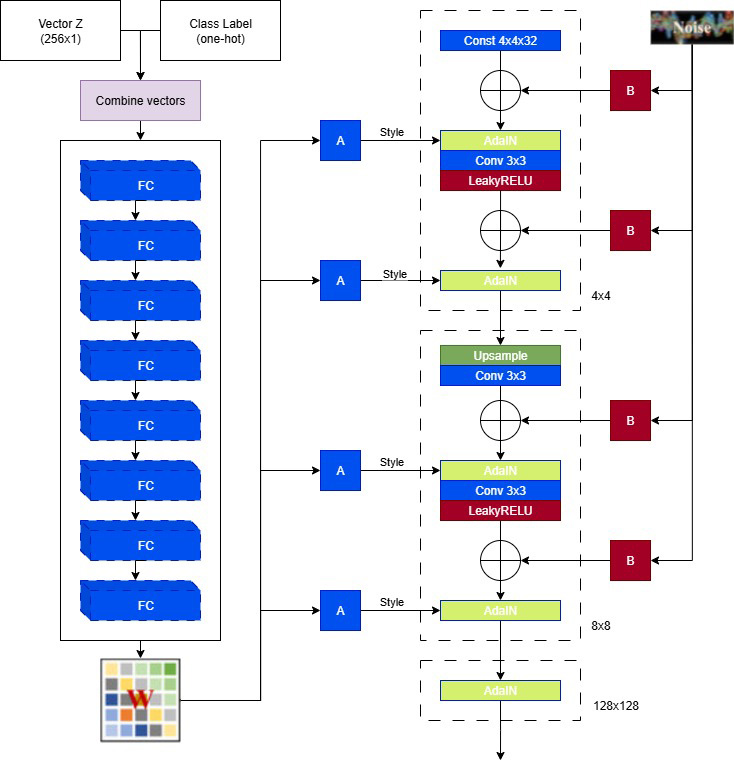
\includegraphics[height=3.6cm]{figures/generator.jpg}
\hfill
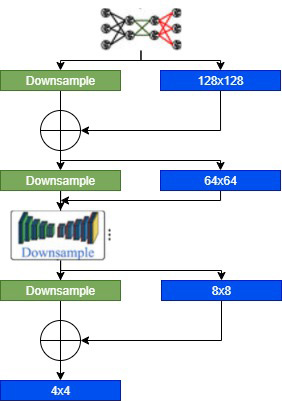
\includegraphics[height=3.6cm]{figures/discriminator.jpg}
\caption{Conditional StyleGAN2-ADA. Left: the style-based generator maps a latent
vector concatenated with the class condition through a mapping network and
AdaIN-modulated blocks. Right: the discriminator receives the (real or synthetic)
image concatenated with the class condition and applies residual convolutional
blocks with $R_1$ regularisation and ADA.}
\label{fig:arch}
\end{figure}

\subsection{Perceptual Selection and Memorisation Audit}
Each generated image's similarity is its \emph{minimum} LPIPS distance to the
DEV reals of the same class. Rather than asserting a threshold, we run a
\textbf{threshold sweep} $\tau\in\{0.10,0.15,0.20,0.25,0.30\}$ and report both
the retained fraction and downstream performance versus $\tau$
(Fig.~\ref{fig:sweep}), making the fidelity--diversity trade-off explicit: a
too-low $\tau$ risks \emph{memorisation} (near-copies of training images); a
too-high $\tau$ admits low-fidelity samples. For retained images we compute the
nearest real neighbour (LPIPS and pixel $L_2$) and \textbf{flag near-copies}
below a small $\epsilon$; the memorisation rate is reported. This directly
addresses the concern that a low perceptual distance can indicate memorisation
rather than fidelity.

\subsection{Generative Fidelity and Diversity (FID, KID)}
Because LPIPS alone cannot detect low diversity or mode collapse, we additionally
report \textbf{FID}~\cite{heusel2017fid} and \textbf{KID}~\cite{binkowski2018kid}
between DEV reals and retained synthetic images, per class. KID (unbiased, with a
variance estimate) is emphasised given the modest sample size.

\subsection{Classifier}
We use \textbf{EfficientNet-B0}~\cite{tan2019efficientnet}, ImageNet-pretrained,
with the head replaced by a single logit and \texttt{BCEWithLogitsLoss}. Input
$128\times128$ RGB with ImageNet normalisation; batch size 32, up to 30 epochs
with early stopping (patience 7) on the inner-DEV validation AUC; train-time
augmentation is horizontal flip and $\pm5^\circ$ rotation. The reported model is
\textbf{fine-tuned end-to-end} (Adam, lr $10^{-4}$); a frozen-backbone variant
that trains only the linear head is near chance on this small $128\times128$ set
(test AUC $\approx 0.55$) and is reported only as an ablation, underscoring that
a functional classifier is needed to measure the augmentation effect. Settings
are in \texttt{configs/finetune.yaml}.

\subsection{Statistical Analysis}
For each ratio we obtain $N_\text{seeds}$ TEST metrics. We report mean, standard
deviation, and a 95\% \textbf{bootstrap confidence interval}; a paired
\textbf{Wilcoxon signed-rank test} against the real-only baseline (same seeds),
\textbf{Holm-corrected} across ratios; \textbf{Cliff's delta} effect size; and
the \textbf{DeLong test}~\cite{delong1988} for AUC differences on the
seed-ensembled TEST predictions. A result is called an improvement only if it is
both consistent and significant after correction.

\subsection{Reproducibility}
All RNGs are seeded (Python/NumPy/PyTorch, deterministic cuDNN). Every stage
writes a JSON run report (config, seeds, git commit, environment, counts,
metrics). Dependencies are pinned. Code and the trained generator checkpoint
(via Git LFS) are released. We follow CLAIM~\cite{mongan2020claim},
TRIPOD+AI~\cite{collins2024tripodai}, and PROBAST+AI~\cite{moons2024probastai}
for dataset description, validation design, risk of bias, and reporting.

% ============================================================================
\section{Results}
% ============================================================================
All numbers below are produced by the powered, leakage-free, patient-level
pipeline (fine-tuned classifier, 10 seeds, locked TEST $n{=}504$).

\subsection{Generative Quality}
Fig.~\ref{fig:samples} shows real, GAN, and diffusion samples for both classes:
the GAN reproduces the global breast shape and coarse tissue texture, while fine
detail is limited at $128\times128$. The synthetic-to-real minimum-LPIPS
distributions per class, and the retention curve versus $\tau$, are shown in
Fig.~\ref{fig:sweep}.

\begin{figure}[t]
\centering
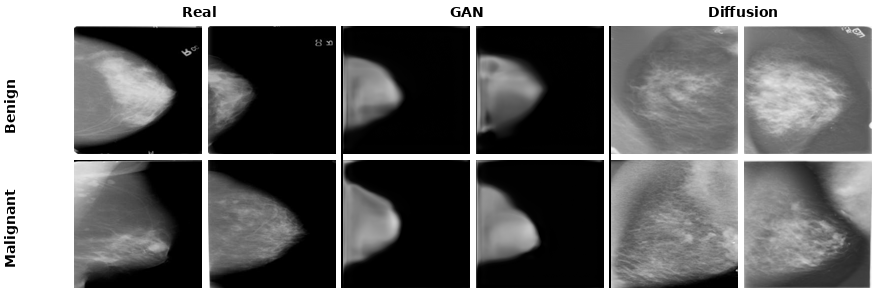
\includegraphics[width=0.82\textwidth]{figures/samples_real_gan_diffusion.png}
\caption{Real, GAN, and diffusion (SD+LoRA) samples for benign (top) and
malignant (bottom) classes. The diffusion generator is more diverse and lower-FID
than the GAN, yet no sample is a near-copy of a real image (memorisation
$0\%$ for both generators).}
\label{fig:samples}
\end{figure} For the GAN we adopt the LPIPS operating point $\tau{=}0.20$, which
retains images of both classes (retained min-LPIPS $\approx 0.18$).
\textbf{No retained sample is a near-copy}: the memorisation rate is $0\%$, far
above the near-copy flag. Distributional fidelity is \emph{limited}---FID
$158.7$ (benign) and $171.6$ (malignant), with correspondingly high KID
(Table~\ref{tab:fidelity})---far from the FID $20$--$60$ typical of strong
mammogram generators, reflecting the difficulty of $128\times128$ synthesis from
a patient-disjoint training set.

\begin{figure}[t]
\centering
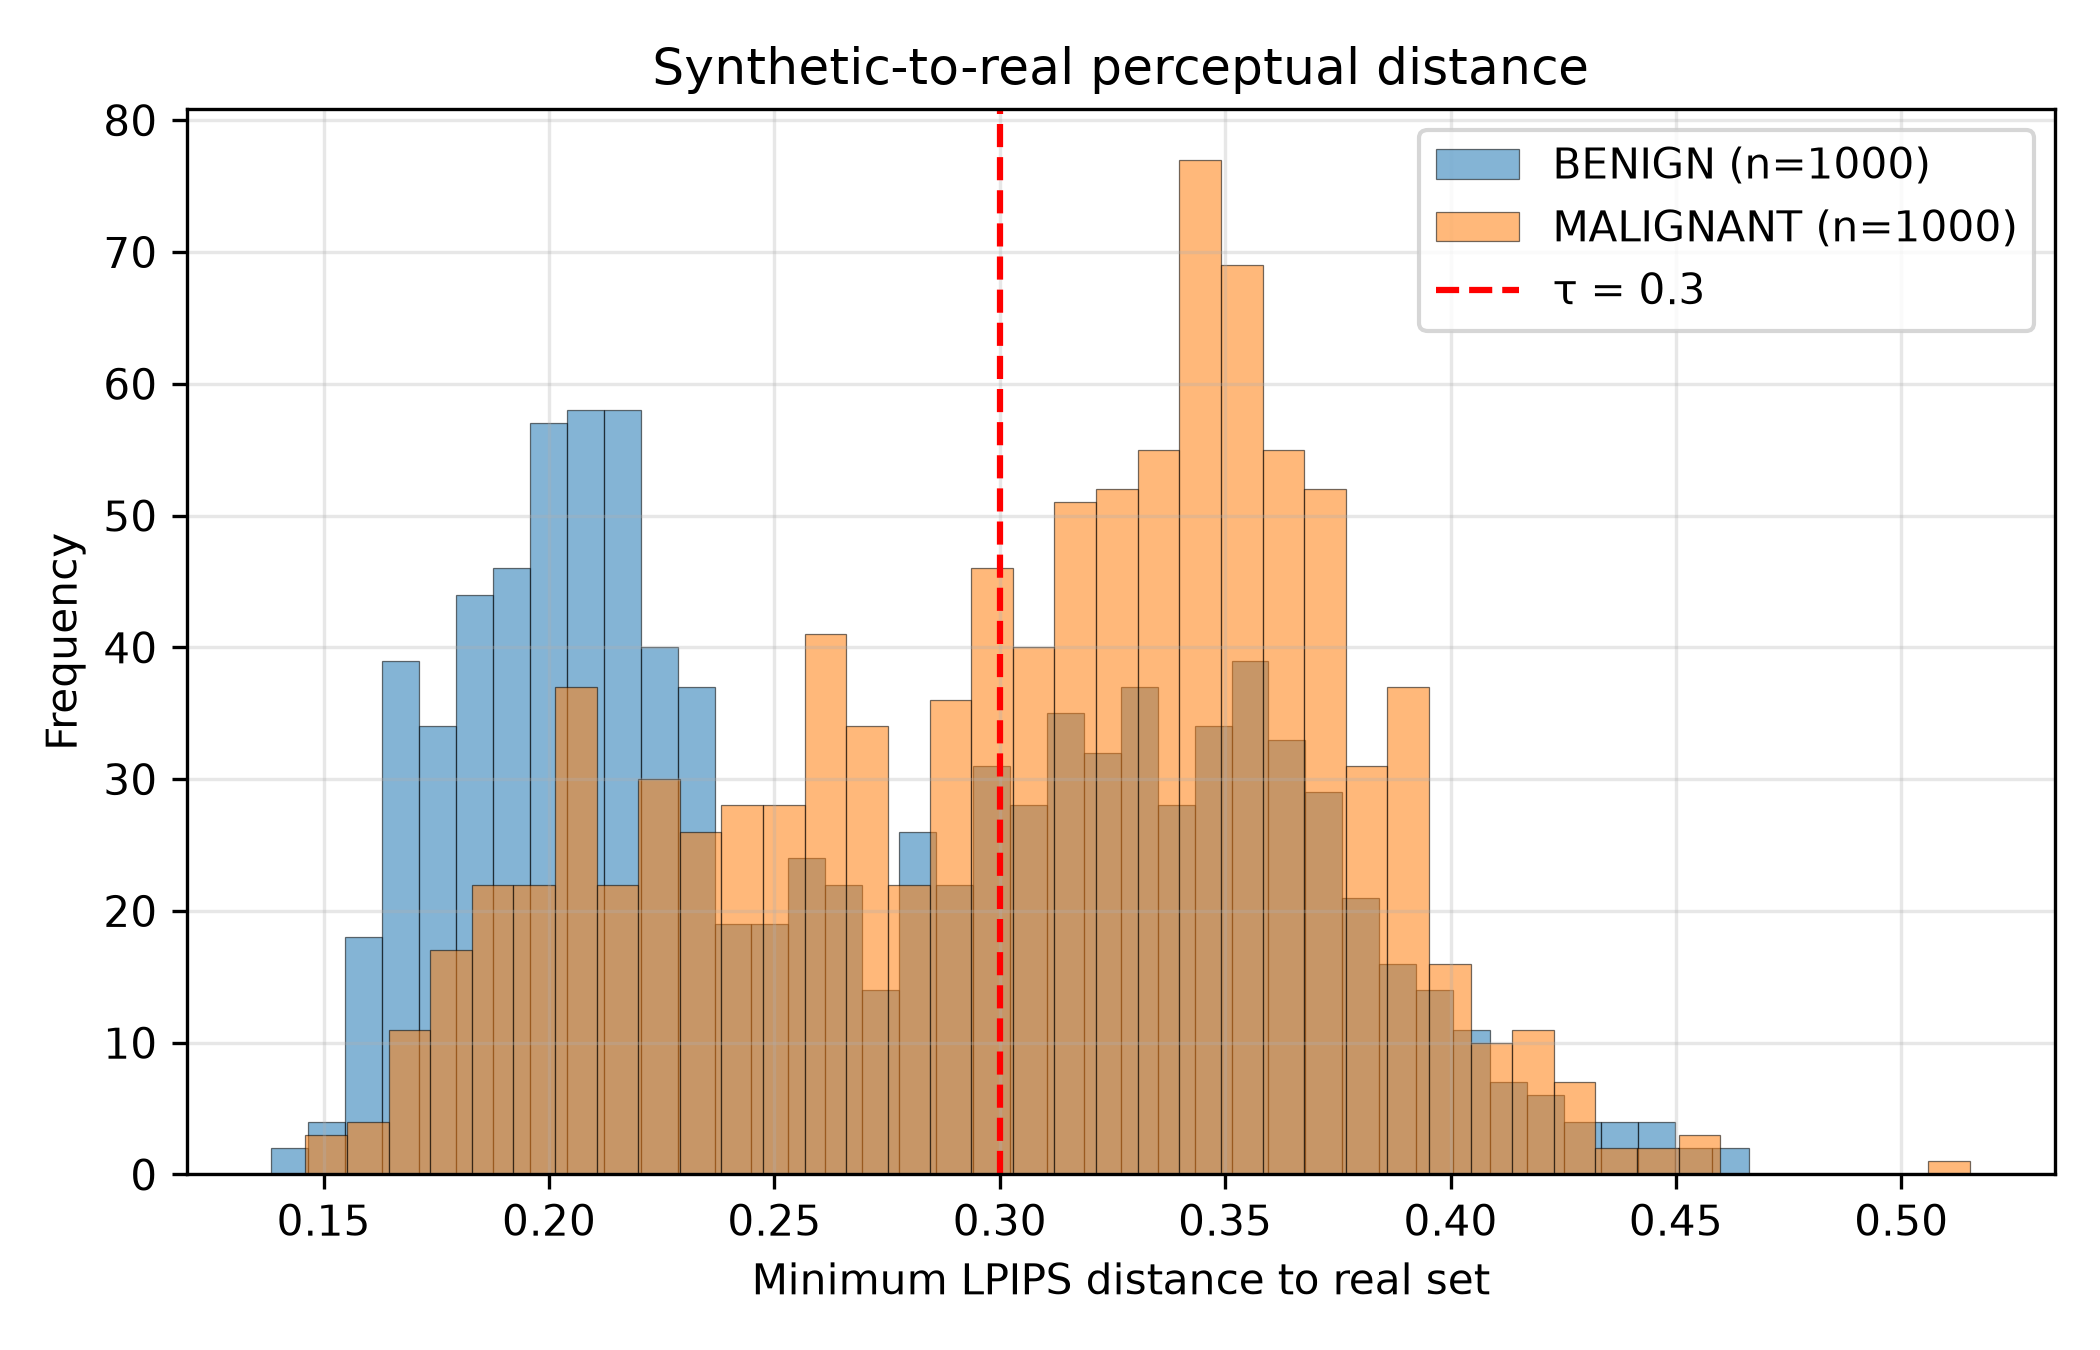
\includegraphics[width=0.48\textwidth]{figures/lpips_distribution.png}
\hfill

\includegraphics[width=0.48\textwidth]{figures/threshold_sweep.png}
\caption{Perceptual selection: synthetic-to-real minimum-LPIPS distribution per
class (left) and the retained fraction versus threshold $\tau$ (right). The sweep
justifies the GAN operating point $\tau{=}0.20$ under the leakage-free,
patient-level generator.}
\label{fig:sweep}
\end{figure}

\begin{table}[t]
\centering
\caption{GAN generative fidelity/diversity between DEV reals and retained
synthetic images (lower is better; GAN selection $\tau{=}0.20$, memorisation
$0\%$). Regenerated by \texttt{scripts/03}.}
\label{tab:fidelity}
\begin{tabular}{lccc}
\toprule
Class & FID $\downarrow$ & KID $\downarrow$ & n (real/fake) \\
\midrule
Benign & 158.7 & 0.175 $\pm$ 0.008 & 1235/4024 \\
Malignant & 171.6 & 0.197 $\pm$ 0.009 & 1006/4024 \\
\bottomrule
\end{tabular}
\end{table}

\subsection{Classification on the Locked Test Set}
Table~\ref{tab:results} reports TEST accuracy, F1, and AUC per synthetic:real
ratio with 95\% bootstrap CIs; Table~\ref{tab:stats} reports the significance
analysis versus the real-only baseline. On the powered dataset the result is
unambiguous and \textbf{negative}: the \emph{real-only} baseline attains the best
AUC ($0.733$), and \textbf{no augmented ratio meaningfully improves on it}
($0.732$--$0.736$ AUC). \textbf{No comparison is statistically significant}: every
Holm-corrected Wilcoxon test fails to reject ($p_\text{adj}{=}1.000$), effect
sizes are negligible (Cliff's $\delta$ from $-0.18$ at 2:1 to $+0.16$ at 4:1),
and the augmented conditions differ from the baseline only within noise. The
95\% CIs of all augmented conditions overlap the baseline
(Fig.~\ref{fig:ratioauc}).

\begin{figure}[t]
\centering

\includegraphics[width=0.62\textwidth]{figures/ratio_auc.png}
\caption{Locked-TEST AUC by synthetic:real ratio (mean over 10 seeds, 95\%
bootstrap CI). No augmented ratio exceeds the real-only baseline; all confidence
intervals overlap, and no difference is statistically significant.}
\label{fig:ratioauc}
\end{figure}

\begin{table}[t]
\centering
\caption{TEST performance by augmentation ratio (mean [95\% CI] over
$N_\text{seeds}$ seeds). Regenerated by \texttt{scripts/04--05}.}
\label{tab:results}
\begin{tabular}{lccc}
\toprule
Synthetic:Real & Accuracy [95\% CI] & F1 [95\% CI] & AUC [95\% CI] \\
\midrule
\textbf{Real only} & \textbf{0.649} [0.643, 0.655] & \textbf{0.642} [0.622, 0.663] & \textbf{0.733} [0.725, 0.740] \\
1:1 & 0.657 [0.644, 0.669] & 0.648 [0.624, 0.670] & 0.732 [0.724, 0.740] \\
2:1 & 0.655 [0.644, 0.667] & 0.663 [0.644, 0.682] & 0.733 [0.724, 0.744] \\
3:1 & 0.645 [0.641, 0.651] & 0.638 [0.624, 0.653] & 0.734 [0.728, 0.738] \\
4:1 & 0.660 [0.652, 0.666] & 0.676 [0.663, 0.689] & 0.736 [0.730, 0.741] \\
\bottomrule
\end{tabular}
\end{table}

\begin{table}[t]
\centering
\caption{Significance of each ratio vs the real-only baseline (AUC).
Holm-corrected Wilcoxon $p$, Cliff's $\delta$, and DeLong $p$. Regenerated by
\texttt{scripts/05}.}
\label{tab:stats}
\begin{tabular}{lcccc}
\toprule
Ratio & Wilcoxon $p_{\text{adj}}$ (AUC) & Cliff's $\delta$ & DeLong $p$ & Signif. \\
\midrule
1:1 & 1.000 & $-0.08$ & 0.473 & no \\
2:1 & 1.000 & $-0.18$ & 0.738 & no \\
3:1 & 1.000 & $+0.06$ & 0.864 & no \\
4:1 & 1.000 & $+0.16$ & 0.978 & no \\
\bottomrule
\end{tabular}
\end{table}

\subsection{Diffusion (SD1.5 + LoRA) vs GAN}
As a state-of-the-art-generator comparison we LoRA-fine-tune Stable
Diffusion 1.5~\cite{rombach2022ldm,hu2022lora} on the DEV images \emph{only}
(leakage-safe), conditioned on per-class prompts, and generate a synthetic set
(best $780$/class by LPIPS). Training runs on a single 8\,GB GPU using fp16 and
gradient checkpointing. The diffusion set is \textbf{more realistic} than the GAN
(FID $131.3$ benign / $126.1$ malignant vs the GAN's $158.7$/$171.6$) and
\textbf{more diverse} (retained min-LPIPS $0.477$/$0.471$, i.e.\ novel rather than
near-copies), with \textbf{zero memorisation} (Table~\ref{tab:diffusion}). Yet
downstream it \textbf{still does not help}: real-only AUC $0.733$; $1{:}1$
$0.732$; $2{:}1$ $0.737$; $3{:}1$ $0.734$; $4{:}1$ $0.725$; all non-significant
(Holm-corrected Wilcoxon $p_\text{adj}$: $1.000$/$1.000$/$1.000$/$0.148$). The
conclusion is pointed: \textbf{improving generator fidelity does not translate
into downstream benefit---generator quality is not the bottleneck}.

\begin{table}[t]
\centering
\caption{GAN vs diffusion (SD+LoRA): the diffusion generator is more realistic
and more diverse with no memorisation, yet neither generator's best ratio beats
the real-only TEST AUC of $0.733$. Regenerated by \texttt{scripts/03--05}.}
\label{tab:diffusion}
\begin{tabular}{lcccc}
\toprule
Generator & FID (benign/malignant) $\downarrow$ & min-LPIPS & Memorised & best TEST AUC \\
\midrule
GAN & 158.7 / 171.6 & 0.18 & 0\% & 0.736 (4:1) \\
Diffusion (SD+LoRA) & 131.3 / 126.1 & 0.47 & 0\% & 0.737 (2:1) \\
\bottomrule
\end{tabular}
\end{table}

\subsection{GAN vs Classic Augmentation}
A GAN is an expensive way to augment data, so a fair question (Reviewer 2) is
whether it beats cheap classic augmentation. Under the same protocol we compare,
against a \emph{no-augmentation} baseline, (i) classic strong augmentation
(affine, photometric jitter, cutout), (ii) GAN synthetic at 2:1, and (iii) both
(Table~\ref{tab:augcompare}). On the powered TEST set all conditions land within
noise of one another: \textbf{GAN augmentation ($0.728$) does not beat classic
augmentation ($0.736$) or even no augmentation ($0.730$)}---the GAN buys nothing
that a few cheap transforms do not, and combining the two does not help. No
comparison is significant (Holm-corrected Wilcoxon, all n.s.).

\begin{table}[t]
\centering
\caption{Augmentation strategies on the locked TEST set (mean [95\% CI], 10
seeds). GAN augmentation does not beat classic augmentation; none differs
significantly from the no-augmentation baseline.}
\label{tab:augcompare}
\begin{tabular}{lcc}
\toprule
Condition & AUC [95\% CI] & vs no-aug. \\
\midrule
No augmentation & 0.730 [0.725, 0.735] & --- \\
Classic aug. & 0.736 [0.729, 0.743] & n.s. \\
GAN 2:1 & 0.728 [0.719, 0.737] & n.s. \\
Classic + GAN 2:1 & 0.731 [0.724, 0.738] & n.s. \\
\bottomrule
\end{tabular}
\end{table}

\subsection{Low-Data Regime}
Synthetic augmentation is often argued to help most when real data is scarce. We
subsample the real DEV pool and compare real-only vs GAN 2:1 at each size
(Fig.~\ref{fig:lc}). The benefit is inconsistent and never significant: at
$100$/class the GAN is slightly \emph{below} real-only ($0.601$ vs $0.610$,
$\Delta{=}-0.009$); the only non-significant hint is at $300$/class ($0.672$ vs
$0.646$, $\Delta{=}+0.026$, $p{=}0.105$); at $600$/class it is again negative
($0.703$ vs $0.712$, $\Delta{=}-0.009$); and at the full $1006$/class it is
negligible ($0.734$ vs $0.738$, $\Delta{=}-0.004$). There is thus no reliable
low-data regime in which the GAN helps under rigorous evaluation.

\begin{figure}[t]
\centering

\includegraphics[width=0.6\textwidth]{figures/learning_curve.png}
\caption{Learning curve: TEST AUC of real-only vs GAN-augmented (2:1) training as
the real DEV pool is subsampled. The GAN provides no consistent or significant
benefit at any data size.}
\label{fig:lc}
\end{figure}

\subsection{External Validation}
To probe generalisation beyond CBIS-DDSM (Reviewer 2), the CBIS-trained
classifier is evaluated \emph{without any retraining} on an independent dataset
(MIAS; 115 abnormal films, 63 benign / 52 malignant, task-matched by excluding
normal films), using the same protocol with the external set in place of the
locked TEST set (Table~\ref{tab:external}). The outcome matches the internal
one and is again \textbf{negative}: the model barely exceeds chance on MIAS
(real-only AUC $0.531$), and augmentation \emph{does not help}---every augmented
ratio sits at or below the real-only baseline ($0.513$--$0.530$), with no
significant difference. The
large domain gap---digitised film versus full-field digital mammography,
different scanner and population, and aggressive $1024\!\to\!128$
downsampling---means the CBIS-trained model does not transfer, and synthetic
augmentation provides no robustness to it. This reinforces that the study is an
exploratory feasibility analysis, not evidence of clinical robustness.

\begin{table}[t]
\centering
\caption{External validation on MIAS (full-CBIS-DDSM-trained model, no
retraining). Every ratio is at or below chance. Regenerated by
\texttt{scripts/06} + \texttt{05}.}
\label{tab:external}
\begin{tabular}{lc}
\toprule
Synthetic:Real & AUC (MIAS) \\
\midrule
Real only & 0.531 \\
1:1 & 0.530 \\
2:1 & 0.522 \\
3:1 & 0.521 \\
4:1 & 0.513 \\
\bottomrule
\end{tabular}
\end{table}

% ============================================================================
\section{Discussion}
% ============================================================================
Under the powered, leakage-free, patient-level protocol, synthetic augmentation
provides \textbf{no measurable benefit for either generator}: the real-only
baseline is the strongest configuration and no augmented ratio is significantly
different from it, whether the synthetic images come from the GAN or from the
diffusion model, and whether evaluated internally or on MIAS. The most
informative result is that the \emph{diffusion} generator---which is more
realistic (lower FID), more diverse, and shows zero memorisation---\emph{still}
yields nothing downstream. \textbf{Generator quality is therefore not the
bottleneck}: raising fidelity from the GAN to a state-of-the-art diffusion model
does not move the classifier.

The leakage story is \textbf{nuanced}. On the full, powered dataset even the
\emph{image-level} (leaky) split, in which same-patient views may straddle train
and test, gives a \textbf{null} result (real-only AUC $0.722$; augmented
$0.721$--$0.736$; all n.s.). The spurious ``significant'' gain of AUC
$0.611\!\to\!0.683$ at 2:1--3:1 (Holm-corrected Wilcoxon $p_\text{adj}{=}0.047$)
appears \textbf{only} on the small $553$-image subset \emph{under} image-level
splitting. In other words, the false positive requires \emph{both} small data
\emph{and} leakage: with adequate power it does not appear even under the leaky
split. This makes the commonly reported gains recoverable as an artefact of the
small-sample-plus-leakage combination, not of the synthetic data.

The augmentation-strategy comparison sharpens the practical message: the GAN
matches, but does not beat, cheap classic augmentation or even no augmentation
(Table~\ref{tab:augcompare}), so its considerable training cost buys no accuracy;
and the low-data analysis (Fig.~\ref{fig:lc}) finds no data size at which the GAN
reliably helps, contrary to the common intuition that synthetic data rescues the
small-sample regime. We do not claim synthetic augmentation \emph{cannot} help
mammography classification; we show that, across two generator families and under
a powered, rigorous evaluation, the commonly reported gains do not reproduce, and
that improving generator fidelity alone is not sufficient to produce one.

% ============================================================================
\section{Limitations}
% ============================================================================
This study reports a powered negative result, not evidence of clinical
robustness. (1) The diffusion generator is built on a \textbf{Stable Diffusion
1.5 base pretrained on natural images}, so a \textbf{domain gap} separates its
prior from mammography; adapting a \emph{medical}-pretrained diffusion base is a
natural avenue for future work, though our finding that fidelity does not drive
downstream benefit tempers the expectation that it would change the conclusion.
(2) $128\times128$ resolution discards fine diagnostic detail (margins, texture,
microcalcifications) and constrains generator quality. (3) External validation
uses a \textbf{single} additional dataset (MIAS, digitised film); broader
multi-institution/multi-scanner validation (INbreast, VinDr-Mammo) remains future
work. (4) Both baseline and augmented AUCs are moderate; the model is not
clinically validated, and no prospective or expert evaluation was performed.
(5) The generators are trained once on DEV in the reported protocol; the
fold-wise variant is provided but not run at scale due to compute.

% ============================================================================
\section{Conclusion}
% ============================================================================
We presented a powered, leakage-free, patient-level protocol (locked TEST
$n{=}504$) for evaluating synthetic augmentation in breast-cancer mammography
classification, with a justified, memorisation-audited selection step, FID/KID
reporting, and full statistical testing, and applied it to \emph{two} generator
families---a StyleGAN2-ADA and a LoRA-fine-tuned Stable Diffusion 1.5. Under this
protocol \textbf{neither generator provides a significant benefit}, internally or
externally. Strikingly, the diffusion generator is more realistic, more diverse,
and free of memorisation, yet still yields nothing downstream---so
\textbf{generator quality is not the bottleneck}. A nuanced ablation shows that
the positive result reported under weaker protocols requires \emph{both} a small
subset \emph{and} image-level leakage; with adequate power it does not appear even
under the leaky split. The contribution is a cautionary, reproducible
demonstration that evaluation rigour and statistical power---not the presence or
fidelity of synthetic data---drive the reported improvements. Future work:
medical-pretrained diffusion bases; higher-resolution generators; multi-scanner
external validation; and the fold-wise protocol at scale.

\subsubsection*{Acknowledgements.} The authors thank the Department of Computing,
State University of Londrina.

\subsubsection*{Data and Code Availability.} Code, configurations, tests, and the
trained generator checkpoint (Git LFS) are released in the project repository.

\bibliographystyle{splncs04}
\bibliography{references}

\end{document}
